\documentclass[11pt,a4paper]{article}
\usepackage{fontspec}
\usepackage{polyglossia}
\setdefaultlanguage{czech}
\usepackage{amsmath,amssymb}
\usepackage{unicode-math}
\setmainfont{Cambria}
\setsansfont{Calibri}
\setmathfont{Cambria Math}
\usepackage[a4paper,margin=2.3cm]{geometry}
\usepackage{graphicx,booktabs,tabularx,float,caption,subcaption,xcolor,enumitem,array}
\usepackage[hidelinks]{hyperref}
\usepackage{tikz}
\usetikzlibrary{arrows.meta,positioning,fit,calc}
\graphicspath{{obrazky/}{../cad/}{../results/}{../results/animace/}}
\captionsetup{font=small,labelfont=bf,labelsep=period}
\setlist{itemsep=2pt,topsep=4pt}
\definecolor{oranz}{HTML}{eb6834}
\definecolor{modra}{HTML}{2a78d6}
\definecolor{seda}{HTML}{52514e}
\definecolor{svetla}{HTML}{f0efec}
\newcommand{\RovinaBezSpicka}{32{,}2}
\newcommand{\RovinaBezSpickaPct}{0}
\newcommand{\RovinaBezSpickaRed}{0}
\newcommand{\RovinaBezFlex}{$-$67{,}1}
\newcommand{\RovinaBezRms}{28{,}9}
\newcommand{\RovinaBezRmsPct}{0}
\newcommand{\RovinaBezRmsRed}{0}
\newcommand{\RovinaBezImpuls}{5{,}4}
\newcommand{\RovinaBezImpulsPct}{0}
\newcommand{\RovinaBezImpulsRed}{0}
\newcommand{\RovinaBezPrace}{16{,}4}
\newcommand{\RovinaBezPracePct}{0}
\newcommand{\RovinaBezPraceRed}{0}
\newcommand{\RovinaBezExoPrace}{0{,}0}
\newcommand{\RovinaBezExoVykon}{0{,}0}
\newcommand{\RovinaPasSpicka}{31{,}9}
\newcommand{\RovinaPasSpickaPct}{$-$1}
\newcommand{\RovinaPasSpickaRed}{1}
\newcommand{\RovinaPasFlex}{$-$67{,}2}
\newcommand{\RovinaPasRms}{28{,}8}
\newcommand{\RovinaPasRmsPct}{$-$0}
\newcommand{\RovinaPasRmsRed}{0}
\newcommand{\RovinaPasImpuls}{5{,}3}
\newcommand{\RovinaPasImpulsPct}{$-$2}
\newcommand{\RovinaPasImpulsRed}{2}
\newcommand{\RovinaPasPrace}{16{,}2}
\newcommand{\RovinaPasPracePct}{$-$1}
\newcommand{\RovinaPasPraceRed}{1}
\newcommand{\RovinaPasExoPrace}{0{,}0}
\newcommand{\RovinaPasExoVykon}{0{,}0}
\newcommand{\RovinaUhelSpicka}{31{,}4}
\newcommand{\RovinaUhelSpickaPct}{$-$2}
\newcommand{\RovinaUhelSpickaRed}{2}
\newcommand{\RovinaUhelFlex}{$-$67{,}2}
\newcommand{\RovinaUhelRms}{30{,}7}
\newcommand{\RovinaUhelRmsPct}{7}
\newcommand{\RovinaUhelRmsRed}{-7}
\newcommand{\RovinaUhelImpuls}{4{,}8}
\newcommand{\RovinaUhelImpulsPct}{$-$12}
\newcommand{\RovinaUhelImpulsRed}{12}
\newcommand{\RovinaUhelPrace}{15{,}5}
\newcommand{\RovinaUhelPracePct}{$-$5}
\newcommand{\RovinaUhelPraceRed}{5}
\newcommand{\RovinaUhelExoPrace}{18{,}3}
\newcommand{\RovinaUhelExoVykon}{234{,}6}
\newcommand{\RovinaCnnSpicka}{31{,}9}
\newcommand{\RovinaCnnSpickaPct}{$-$1}
\newcommand{\RovinaCnnSpickaRed}{1}
\newcommand{\RovinaCnnFlex}{$-$67{,}2}
\newcommand{\RovinaCnnRms}{28{,}8}
\newcommand{\RovinaCnnRmsPct}{$-$0}
\newcommand{\RovinaCnnRmsRed}{0}
\newcommand{\RovinaCnnImpuls}{5{,}3}
\newcommand{\RovinaCnnImpulsPct}{$-$2}
\newcommand{\RovinaCnnImpulsRed}{2}
\newcommand{\RovinaCnnPrace}{16{,}2}
\newcommand{\RovinaCnnPracePct}{$-$1}
\newcommand{\RovinaCnnPraceRed}{1}
\newcommand{\RovinaCnnExoPrace}{0{,}0}
\newcommand{\RovinaCnnExoVykon}{0{,}0}
\newcommand{\RovinaIdealSpicka}{31{,}9}
\newcommand{\RovinaIdealSpickaPct}{$-$1}
\newcommand{\RovinaIdealSpickaRed}{1}
\newcommand{\RovinaIdealFlex}{$-$67{,}2}
\newcommand{\RovinaIdealRms}{28{,}8}
\newcommand{\RovinaIdealRmsPct}{$-$0}
\newcommand{\RovinaIdealRmsRed}{0}
\newcommand{\RovinaIdealImpuls}{5{,}3}
\newcommand{\RovinaIdealImpulsPct}{$-$2}
\newcommand{\RovinaIdealImpulsRed}{2}
\newcommand{\RovinaIdealPrace}{16{,}2}
\newcommand{\RovinaIdealPracePct}{$-$1}
\newcommand{\RovinaIdealPraceRed}{1}
\newcommand{\RovinaIdealExoPrace}{0{,}0}
\newcommand{\RovinaIdealExoVykon}{0{,}0}
\newcommand{\SchodyBezSpicka}{161{,}8}
\newcommand{\SchodyBezSpickaPct}{0}
\newcommand{\SchodyBezSpickaRed}{0}
\newcommand{\SchodyBezFlex}{$-$56{,}8}
\newcommand{\SchodyBezRms}{59{,}6}
\newcommand{\SchodyBezRmsPct}{0}
\newcommand{\SchodyBezRmsRed}{0}
\newcommand{\SchodyBezImpuls}{37{,}9}
\newcommand{\SchodyBezImpulsPct}{0}
\newcommand{\SchodyBezImpulsRed}{0}
\newcommand{\SchodyBezPrace}{71{,}6}
\newcommand{\SchodyBezPracePct}{0}
\newcommand{\SchodyBezPraceRed}{0}
\newcommand{\SchodyBezExoPrace}{0{,}0}
\newcommand{\SchodyBezExoVykon}{0{,}0}
\newcommand{\SchodyPasSpicka}{162{,}0}
\newcommand{\SchodyPasSpickaPct}{0}
\newcommand{\SchodyPasSpickaRed}{-0}
\newcommand{\SchodyPasFlex}{$-$56{,}4}
\newcommand{\SchodyPasRms}{59{,}6}
\newcommand{\SchodyPasRmsPct}{0}
\newcommand{\SchodyPasRmsRed}{-0}
\newcommand{\SchodyPasImpuls}{37{,}9}
\newcommand{\SchodyPasImpulsPct}{0}
\newcommand{\SchodyPasImpulsRed}{-0}
\newcommand{\SchodyPasPrace}{71{,}9}
\newcommand{\SchodyPasPracePct}{0}
\newcommand{\SchodyPasPraceRed}{-0}
\newcommand{\SchodyPasExoPrace}{0{,}0}
\newcommand{\SchodyPasExoVykon}{0{,}0}
\newcommand{\SchodyUhelSpicka}{112{,}5}
\newcommand{\SchodyUhelSpickaPct}{$-$30}
\newcommand{\SchodyUhelSpickaRed}{30}
\newcommand{\SchodyUhelFlex}{$-$56{,}4}
\newcommand{\SchodyUhelRms}{42{,}2}
\newcommand{\SchodyUhelRmsPct}{$-$29}
\newcommand{\SchodyUhelRmsRed}{29}
\newcommand{\SchodyUhelImpuls}{25{,}4}
\newcommand{\SchodyUhelImpulsPct}{$-$33}
\newcommand{\SchodyUhelImpulsRed}{33}
\newcommand{\SchodyUhelPrace}{54{,}9}
\newcommand{\SchodyUhelPracePct}{$-$23}
\newcommand{\SchodyUhelPraceRed}{23}
\newcommand{\SchodyUhelExoPrace}{18{,}3}
\newcommand{\SchodyUhelExoVykon}{79{,}5}
\newcommand{\SchodyCnnSpicka}{122{,}1}
\newcommand{\SchodyCnnSpickaPct}{$-$25}
\newcommand{\SchodyCnnSpickaRed}{25}
\newcommand{\SchodyCnnFlex}{$-$56{,}4}
\newcommand{\SchodyCnnRms}{44{,}2}
\newcommand{\SchodyCnnRmsPct}{$-$26}
\newcommand{\SchodyCnnRmsRed}{26}
\newcommand{\SchodyCnnImpuls}{26{,}1}
\newcommand{\SchodyCnnImpulsPct}{$-$31}
\newcommand{\SchodyCnnImpulsRed}{31}
\newcommand{\SchodyCnnPrace}{53{,}1}
\newcommand{\SchodyCnnPracePct}{$-$26}
\newcommand{\SchodyCnnPraceRed}{26}
\newcommand{\SchodyCnnExoPrace}{19{,}2}
\newcommand{\SchodyCnnExoVykon}{100{,}9}
\newcommand{\SchodyIdealSpicka}{122{,}1}
\newcommand{\SchodyIdealSpickaPct}{$-$25}
\newcommand{\SchodyIdealSpickaRed}{25}
\newcommand{\SchodyIdealFlex}{$-$56{,}4}
\newcommand{\SchodyIdealRms}{44{,}0}
\newcommand{\SchodyIdealRmsPct}{$-$26}
\newcommand{\SchodyIdealRmsRed}{26}
\newcommand{\SchodyIdealImpuls}{26{,}3}
\newcommand{\SchodyIdealImpulsPct}{$-$31}
\newcommand{\SchodyIdealImpulsRed}{31}
\newcommand{\SchodyIdealPrace}{54{,}6}
\newcommand{\SchodyIdealPracePct}{$-$24}
\newcommand{\SchodyIdealPraceRed}{24}
\newcommand{\SchodyIdealExoPrace}{17{,}3}
\newcommand{\SchodyIdealExoVykon}{94{,}7}
\newcommand{\CnnCistaF}{0{,}991}
\newcommand{\CnnCistaPrec}{0{,}983}
\newcommand{\CnnCistaRec}{1{,}000}
\newcommand{\CnnCistaAcc}{0{,}997}
\newcommand{\CnnSumF}{0{,}979}
\newcommand{\CnnSumPrec}{0{,}974}
\newcommand{\CnnSumRec}{0{,}983}
\newcommand{\CnnSumAcc}{0{,}993}
\newcommand{\CnnPomalaF}{0{,}963}
\newcommand{\CnnPomalaPrec}{0{,}929}
\newcommand{\CnnPomalaRec}{1{,}000}
\newcommand{\CnnPomalaAcc}{0{,}987}
\newcommand{\CnnRychlaF}{0{,}952}
\newcommand{\CnnRychlaPrec}{0{,}909}
\newcommand{\CnnRychlaRec}{1{,}000}
\newcommand{\CnnRychlaAcc}{0{,}983}
\newcommand{\CnnParam}{2533}
\newcommand{\CnnOken}{70411}
\newcommand{\CnnPodilOn}{12}
\newcommand{\CnnEpochy}{40}
\newcommand{\CnnZpozdeniOn}{10}
\newcommand{\CnnZpozdeniOff}{20}
\newcommand{\CnnFalesna}{0}

\newcommand{\Nm}{\,N\,m}
\newcommand{\pct}{\,\%}

\title{\textbf{Exoskelet pravého kolene pro výstup do schodů}\\[4pt]
\large Model v OpenSim, řízení motoru konvoluční neuronovou sítí\\a vyhodnocení odlehčení kolene}
\author{}
\date{13. října 2026}

\begin{document}
\maketitle
\thispagestyle{empty}

\begin{abstract}
\noindent
Zpráva popisuje simulaci chůze po rovině a výstupu do schodů (15\,m, model 72,6\,kg)
v programu OpenSim, na kterou je doplněn exoskelet pravého kolene. Exoskelet je navržen jako
parametrický CAD model (1,76\,kg, laterální pohon s vlnovým převodem). Motor se zapíná a vypíná
konvoluční neuronovou sítí, která každých 50\,ms (20\,Hz) vyhodnotí poslední 1\,s signálů
úhlu kolene a úhlových rychlostí stehna a holeně. Síť se učila z momentu v koleni při běžné chůzi:
motor má běžet tehdy, když extenzní moment kolene na schodech překročí 40\Nm.
Na rovině se motor nezapnul ani jednou. Při výstupu do schodů exoskelet snížil
špičku extenzního momentu, který musí vyvinout svaly kolene, z \SchodyBezSpicka\Nm{} na
\SchodyCnnSpicka\Nm{} (\SchodyCnnSpickaPct\pct), extenzní impuls o \SchodyCnnImpulsRed\pct{}
a kladnou mechanickou práci svalů kolene z \SchodyBezPrace\,J na \SchodyCnnPrace\,J na krok
(\SchodyCnnPracePct\pct).
\end{abstract}

\tableofcontents
\newpage

%==========================================================================
\section{Úvod a cíle}

Výchozím bodem je simulace z projektu \texttt{test1}: model
\emph{Gait10dof18musc} (OpenSim 4.5) projde 10,6\,m po rovině a vystoupá 17 schodů
170/290\,mm. Pro pravou nohu jsou známé kloubní úhly a momenty v kyčli, koleni a kotníku.
Nejvíce zatížené je koleno při výstupu do schodů, kde extenzní moment dosahuje přibližně
160\Nm{} (2,2\Nm/kg). V projektu \texttt{test2} jsou přidány:

\begin{enumerate}
  \item exoskelet pravého kolene jako CAD model, včetně hmotnosti a setrvačnosti v modelu (kap.~\ref{sec:cad}),
  \item řízení motoru konvoluční neuronovou sítí s výstupem zapnuto/vypnuto (kap.~\ref{sec:cnn}),
  \item vyhodnocení, jak exoskelet odlehčí koleno (kap.~\ref{sec:vysledky}),
  \item animace chůze, ve které kamera sleduje model (kap.~\ref{sec:animace}).
\end{enumerate}

Kapitola~\ref{sec:opensim} nejprve vysvětluje, co model v OpenSim počítá. Bez toho nelze
výsledky správně interpretovat.

%==========================================================================
\section{Jak funguje model v OpenSim}\label{sec:opensim}

\subsection{Muskuloskeletální model}

Model \emph{Gait10dof18musc} je soustava tuhých těles (segmentů těla) spojených klouby.
Jde o rovinný (sagitální) model, takže pohyb probíhá jen ve svislé rovině ve směru chůze.

\begin{table}[H]
\centering\small
\begin{tabularx}{\textwidth}{lX}
\toprule
Tělesa (12) & pánev, trup s hlavou a rukama, 2× stehenní kost, 2× holeň, 2× hlezenní kost,
              2× pata, 2× prsty (s exoskeletem navíc 2 články exo)\\
Stupně volnosti (10) & náklon pánve, vodorovná a svislá poloha pánve; flexe kyčle, kolene
              a kotníku vpravo i vlevo; extenze bederní páteře\\
Koleno & \texttt{CustomJoint}: rotace kolem příčné osy, k níž je přes splajny vázán posuv holeně
              o několik milimetrů (valení a klouzání kondylů); osa otáčení tedy není pevná\\
Svaly (18) & 9 na každé noze; ve výpočtu momentů se nepoužívají (viz níže)\\
Hmotnost & 72,6\,kg (s exoskeletem 74,4\,kg)\\
\bottomrule
\end{tabularx}
\caption{Složení modelu.}
\end{table}

\subsection{Pohybové rovnice}

Polohu celého těla popisuje vektor zobecněných souřadnic $\mathbf q$ (10 hodnot). Pohybové
rovnice soustavy tuhých těles mají tvar
\begin{equation}
  \mathbf M(\mathbf q)\,\ddot{\mathbf q} \;+\; \mathbf c(\mathbf q,\dot{\mathbf q})
  \;+\; \mathbf g(\mathbf q)
  \;=\; \boldsymbol\tau \;+\; \mathbf J^{\mathsf T}(\mathbf q)\,\mathbf F_{\text{GRF}}
  \;+\; \boldsymbol\tau_{\text{exo}},
  \label{eq:eom}
\end{equation}
kde $\mathbf M$ je matice hmotnosti, $\mathbf c$ obsahuje odstředivé a Coriolisovy síly,
$\mathbf g$ tíhu, $\boldsymbol\tau$ jsou čisté momenty v kloubech, které vytvářejí svaly
(tzv. \emph{net joint moments}), $\mathbf F_{\text{GRF}}$ jsou reakční síly země působící
na chodidla, $\mathbf J$ jejich Jacobián a $\boldsymbol\tau_{\text{exo}}$ je moment motoru
exoskeletu (nenulový jen ve složce kolene).

\subsection{Inverzní dynamika – dynamika s předepsanou kinematikou}

\textbf{Ano, model počítá dynamiku s předepsanou kinematikou.} V OpenSim se tato
úloha jmenuje \emph{inverzní dynamika} (nástroj \texttt{InverseDynamicsTool}). Pohyb
$\mathbf q(t)$ je předem zadaný a nástroj ho nepočítá. Rychlosti $\dot{\mathbf q}$ a zrychlení
$\ddot{\mathbf q}$ se získají derivací zadaného pohybu. Reakční síly země se zadají jako vnější
síly. Rovnice~\eqref{eq:eom} se pak v každém časovém okamžiku řeší algebraicky pro neznámé
momenty $\boldsymbol\tau$:
\begin{equation}
  \boldsymbol\tau(t) = \mathbf M\ddot{\mathbf q} + \mathbf c + \mathbf g
  - \mathbf J^{\mathsf T}\mathbf F_{\text{GRF}} - \boldsymbol\tau_{\text{exo}} .
  \label{eq:id}
\end{equation}
Nic se neintegruje v čase a výsledek v jednom okamžiku nezávisí na ostatních okamžicích.
Pánev nemá žádný sval ani motor, takže její tři „momenty“ by měly vyjít nulové. Jsou to
\emph{zbytkové síly}, které ukazují, jak dobře k sobě sedí pohyb a reakční síly.
Na schodech vyšly 0\,N, 0\,N a 1,8\Nm{} RMS. Na rovině s naměřenými daty jsou
typicky 10--20\,N, což je běžná hodnota.

\begin{figure}[H]
\centering
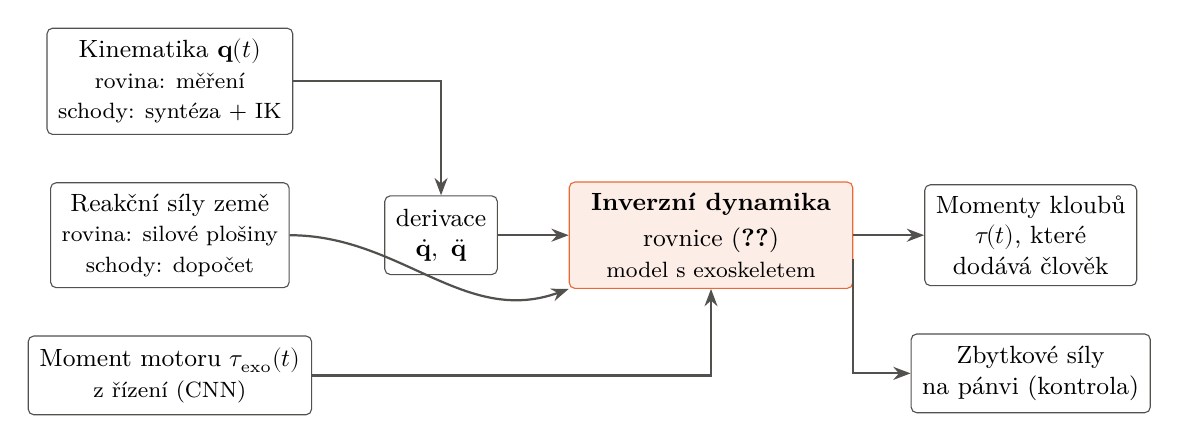
\begin{tikzpicture}[
  box/.style={draw=seda,rounded corners=2pt,align=center,font=\small,minimum height=1.0cm,inner sep=4pt,fill=white},
  hl/.style={box,fill=oranz!12,draw=oranz},
  ar/.style={-{Stealth[length=2.2mm]},seda,thick},
  node distance=6mm and 9mm]
\node[box] (kin) {Kinematika $\mathbf q(t)$\\\footnotesize rovina: měření\\\footnotesize schody: syntéza + IK};
\node[box,below=of kin] (grf) {Reakční síly země\\\footnotesize rovina: silové plošiny\\\footnotesize schody: dopočet};
\node[box,below=of grf] (exo) {Moment motoru $\tau_{\text{exo}}(t)$\\\footnotesize z řízení (CNN)};
\node[box,right=12mm of grf] (fil) {derivace\\$\dot{\mathbf q},\ \ddot{\mathbf q}$};
\node[hl,right=9mm of fil,minimum width=3.6cm] (id) {\textbf{Inverzní dynamika}\\[2pt] rovnice \eqref{eq:id}\\\footnotesize model s exoskeletem};
\node[box,right=9mm of id] (out) {Momenty kloubů\\$\boldsymbol\tau(t)$, které\\dodává člověk};
\node[box,below=of out] (res) {Zbytkové síly\\na pánvi (kontrola)};
\draw[ar] (kin) -| (fil);
\draw[ar] (fil) -- (id);
\draw[ar] (grf.east) to[out=0,in=200] (id.south west);
\draw[ar] (exo.east) -| (id.south);
\draw[ar] (id) -- (out);
\draw[ar] (id.east) ++(0,-0.3) |- (res);
\end{tikzpicture}
\caption{Tok dat ve výpočtu. Pohyb je vstupem, ne výsledkem; počítají se síly a momenty,
které daný pohyb vyžaduje.}
\label{fig:tok}
\end{figure}

\subsection{Odkud pochází pohyb a reakční síly}
\begin{itemize}
  \item \textbf{Rovina (0--8,6\,s):} naměřená chůze z ukázkových dat OpenSim (1,13\,m/s,
        snímání markerů + silové plošiny), převedená z běžeckého pásu na chůzi po zemi
        a sedmkrát zopakovaná. Všech šest vyhodnocovaných cyklů na rovině je proto stejných.
  \item \textbf{Schody:} pohyb není naměřený, ale \emph{syntetický}. Chodidla se kladou
        na stupně, pánev se v každém kroku zvedne o výšku stupně a úhly kloubů se dopočtou
        inverzní kinematikou. Reakční síly se dopočtou z dynamiky celého těla. Metoda byla ověřena
        na rovině proti silovým plošinám (moment kolene: korelace $r=0{,}96$).
  \item Kinematika je vyhlazená filtrem 6\,Hz. Extenzní moment kolene na schodech
        (2,2\Nm/kg) je proti literatuře (1,0--1,6\Nm/kg) spíše nadhodnocený, takže pro dimenzování
        je to konzervativní odhad.
\end{itemize}

\subsection{Co z toho plyne pro exoskelet}
Exoskelet ovlivní výpočet dvěma způsoby:
\begin{enumerate}
  \item \textbf{Hmotností} (1,76\,kg na pravé noze). Mění se $\mathbf M$, $\mathbf g$ i potřebné reakční
        síly. Proto je výpočet zopakován s modelem, který obsahuje exoskelet (kap.~\ref{sec:pripojeni}).
  \item \textbf{Momentem motoru} $\tau_{\text{exo}}$. Rovnice~\eqref{eq:id} je v něm
        lineární, takže moment kolene, který musí dodat člověk, je
        \begin{equation}
          M_{\text{člověk}}(t) = M_{\text{pasivní exo}}(t) - \tau_{\text{exo}}(t).
          \label{eq:superpozice}
        \end{equation}
        Pro předepsaný pohyb to platí přesně. Ověřeno bylo i v OpenSim: řízení bylo zapsáno
        přímo do modelu (\texttt{ExpressionBasedCoordinateForce}) a výsledek se od
        rovnice~\eqref{eq:superpozice} lišil nejvýše o 0,06\Nm.
\end{enumerate}

\noindent\textbf{Důležitý předpoklad:} pohyb člověka je s exoskeletem i bez něj \emph{stejný}.
Model tedy odpovídá na otázku: „Kolik musí dodat svaly, když exoskelet pomáhá a člověk chodí stejně?“
Případnou adaptaci chůze, například jiné úhly nebo rychlost, inverzní dynamika ze své podstaty neukáže.

\subsection{Rozdíl oproti dopředné simulaci}
Při \emph{dopředné} dynamice se z rovnice~\eqref{eq:eom} počítá zrychlení
$\ddot{\mathbf q} = \mathbf M^{-1}(\boldsymbol\tau + \mathbf J^{\mathsf T}\mathbf F + \boldsymbol\tau_{\text{exo}} - \mathbf c - \mathbf g)$
a integruje se v čase. Pohyb je pak výsledkem. K tomu je ale potřeba znát buzení všech svalů
(nástroje CMC, Static Optimization, OpenSim Moco) a mít model kontaktu chodidla se zemí.
Bez toho model upadne. Pro posouzení odlehčení kolene při známém pohybu je inverzní dynamika
standardní a robustní volba. Dopředná simulace je přirozeným dalším krokem, pokud nás zajímá,
jak se chůze s exoskeletem změní.

%==========================================================================
\section{Exoskelet: CAD model a začlenění do OpenSim}\label{sec:cad}

\subsection{Konstrukce}
Exoskelet je navržen parametricky v Pythonu. Rozměry jsou v souboru \texttt{exo\_params.py}.
Díly jsou uzavřené trojúhelníkové sítě vytvořené tažením průřezů. Z nich se počítá objem,
těžiště a tenzor setrvačnosti (Gaussova věta po čtyřstěnech) a exportují se do STL.

\begin{figure}[H]
\centering
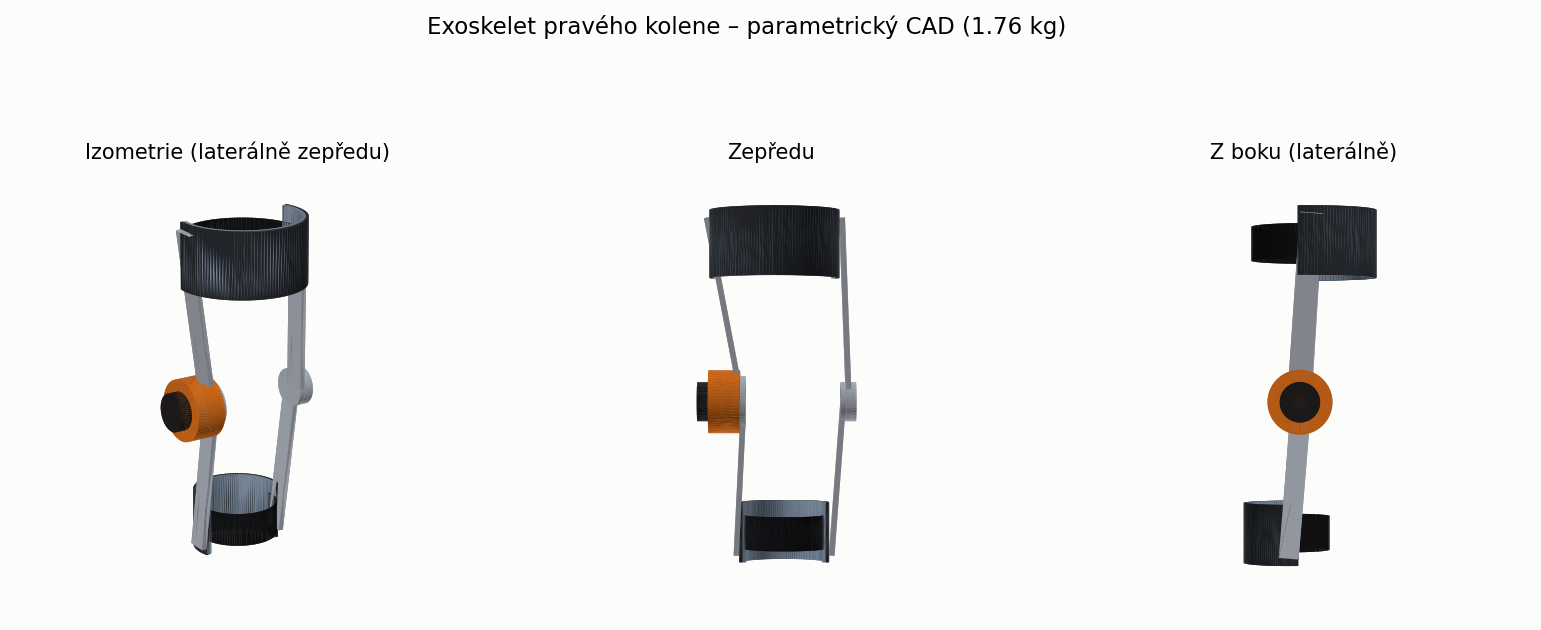
\includegraphics[width=\textwidth]{exo_nahled.png}
\caption{CAD model exoskeletu pravého kolene. Oranžově pohon (BLDC motor s vlnovým převodem),
šedě hliníková ramena, tmavě kompozitové objímky, černě textilní pásky.}
\end{figure}

\begin{itemize}
  \item \textbf{Oboustranné uspořádání:} laterálně je pohon (0,72\,kg) s elektronikou (0,10\,kg),
        mediálně pasivní kloub s ložiskem. Ramena jsou z hliníku 7075, tloušťka 7\,mm.
  \item \textbf{Objímky:} na stehně přední kompozitová skořepina se zadním páskem, na bérci
        zadní skořepina na lýtku s předním páskem. Pro extenzní moment je to správné uspořádání:
        exoskelet tlačí na stehno zepředu a na lýtko zezadu. Pod skořepinou je 5\,mm pěnová
        výstelka.
  \item \textbf{Hmotnost:} článek stehna 1,34\,kg, článek bérce 0,42\,kg, celkem 1,76\,kg.
        Podrobný kusovník je v \texttt{cad/kusovnik.md}.
\end{itemize}

\begin{figure}[H]
\centering
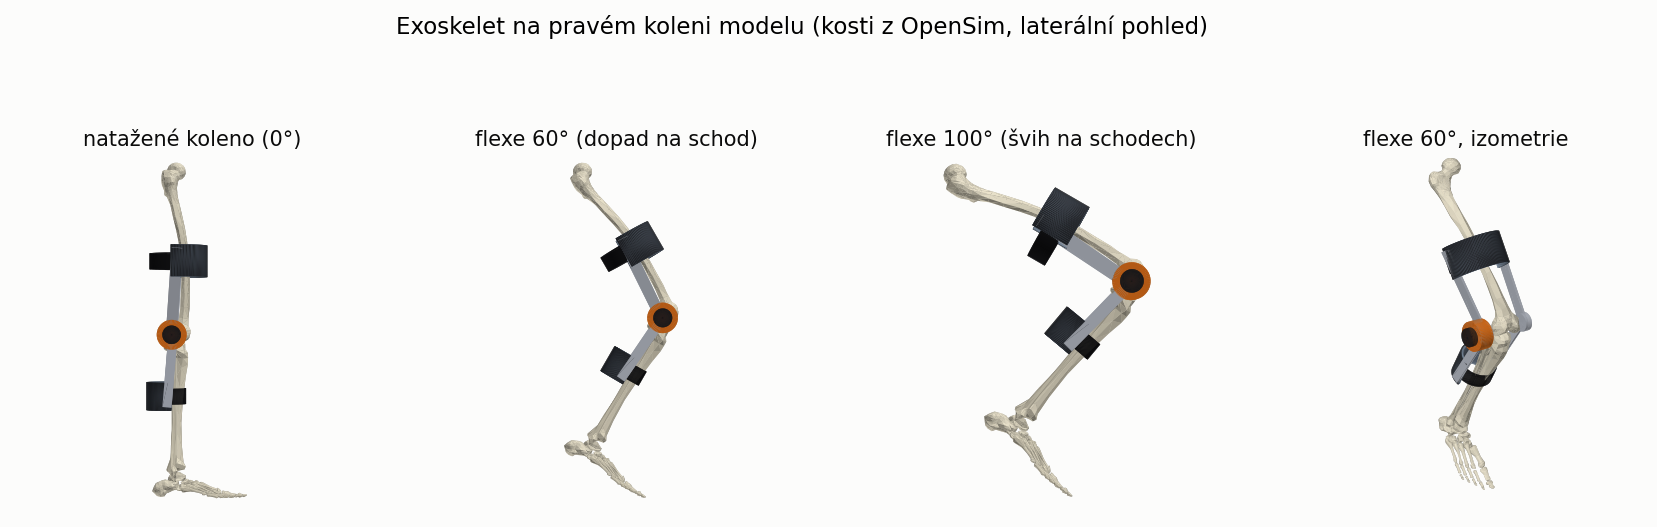
\includegraphics[width=\textwidth]{exo_na_noze.png}
\caption{Exoskelet na kostře modelu při flexi kolene 0°, 60° a 100°.}
\end{figure}

\subsection{Poloha osy kloubu}
Koleno modelu nemá pevnou osu otáčení. Pevný kloub exoskeletu proto nemůže sedět přesně.
Osa byla umístěna metodou nejmenších čtverců tak, aby se její poloha vůči holeni v rozsahu
flexe 0--110° měnila co nejméně. Leží přibližně 8\,mm za počátkem holeně a 15\,mm pod ním
(při natažené noze). Zbytková nesouosost je nejvýše 2,0\,mm (RMS 0,8\,mm). Kdyby osa byla
v počátku holeně, odchylka by byla až 28\,mm, a takový rozdíl by se projevil posouváním objímek
po kůži.

\subsection{Připojení k modelu a reakční síly}\label{sec:pripojeni}
Oba články jsou ke stehenní kosti a holeni připojeny pevně (\texttt{WeldJoint}). To odpovídá
dobře dotaženým objímkám. Moment motoru působí na souřadnici kolene \texttt{knee\_angle\_r}.
Protože exoskelet přidá hmotu, musí se změnit i reakční síly země. K původním silám se přičte
síla potřebná na nesení a zrychlování exoskeletu a rozdělí se mezi chodidla podle jejich
svislého zatížení. Působiště se posune nejvýše o 34\,mm (RMS 9\,mm). Zbytkové síly na pánvi
pak zůstanou stejné jako bez exoskeletu.
Samotná hmota exoskeletu změní špičky momentu kolene o méně než 1\Nm{}
(okamžitě nejvýše o 5\Nm{} ve švihu), ze silového hlediska je tedy zanedbatelná.

%==========================================================================
\section{Řízení motoru konvoluční neuronovou sítí}\label{sec:cnn}

\subsection{Zadání}
\begin{itemize}
  \item \textbf{Výstup:} motor zapnut/vypnut. Zapnutý motor dává extenzní moment 40\Nm{}
        a náběh momentu má časovou konstantu 20\,ms.
  \item \textbf{Vstup:} posledních 1\,s tří signálů vzorkovaných 20\,Hz, tedy okno $3\times20$:
        flexe kolene (enkodér v kloubu exoskeletu) a úhlová rychlost stehna a holeně vůči zemi
        (gyroskopy IMU na objímkách; kladná hodnota = otáčení segmentu dopředu).
  \item \textbf{Rozhodnutí} se počítá každých 50\,ms a drží se do dalšího vzorku.
        Okno obsahuje jen minulá data, takže řízení je kauzální a lze ho realizovat v reálném čase.
  \item \textbf{Pomáhá se jen do schodů.} Na rovině má motor zůstat vypnutý.
\end{itemize}

\subsection{Trénovací data a štítky}
Štítky (správné odpovědi) se odvozují z momentu kolene při běžné chůzi bez exoskeletu:
\begin{equation}
  \text{ON}(t) \iff M_{\text{koleno}}(t) > 40\,\text{N\,m} \;\wedge\; \text{pravá noha stojí na schodu}.
\end{equation}
Práh 40\Nm{} je stejný jako moment zapnutého motoru. Exoskelet tedy pomáhá jen tehdy, když
potřebný moment je alespoň tak velký jako moment motoru, a v ideálním případě nikdy nepůsobí
proti člověku. Na rovině se moment k prahu jen přiblíží (32\Nm, při přechodu na schody krátce 42\Nm). Podmínka
„stojí na schodu“ ale zaručuje, že na rovině je štítek vždy OFF. Na schodech je motor ON
asi 0,29\,s v každém kroku, tj. přibližně 22\pct{} času. Moment kolene se jako vstup síti
\emph{nedává}, protože ho nelze přímo měřit. Síť se musí naučit poznat situaci
ze snímatelných veličin.

\textbf{Rozdělení dat.} Data mají 200\,Hz, síť pracuje s 20\,Hz. Podvzorkování s deseti různými
fázemi tak dává deset různých posloupností. Poslední cyklus roviny a poslední dva kroky
na schodech tvoří \emph{testovací množinu}. Do učení nevstupují, a to ani okna, která
by je zasahovala.

\textbf{Augmentace.} Měřená i syntetická chůze má málo variability (cykly se opakují),
proto se z trénovací části vytvoří 240 variant:
změna rychlosti chůze $\pm15$\pct{} (časové škálování; úhlové rychlosti se škálují s ní),
zesílení kanálů $\pm10$\pct, offset úhlu (σ = 2°), bias gyroskopů (σ = 5\,°/s) a bílý šum
(0,5° a 6\,°/s). Tak vzniklo \CnnOken{} trénovacích oken, z toho \CnnPodilOn\pct{} ON.

\subsection{Architektura}
\begin{figure}[H]
\centering
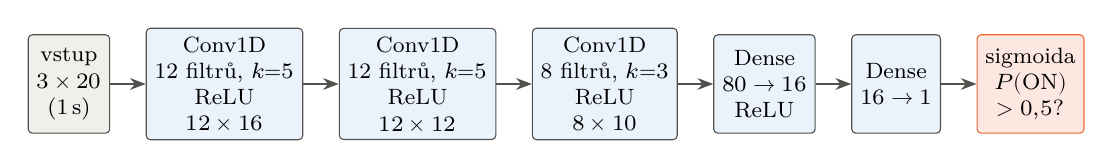
\begin{tikzpicture}[
  l/.style={draw=seda,fill=modra!10,rounded corners=1.5pt,align=center,font=\footnotesize,minimum height=1.25cm,inner sep=3pt},
  o/.style={l,fill=oranz!15,draw=oranz},
  ar/.style={-{Stealth[length=2mm]},seda},
  node distance=4.5mm]
\node[l,fill=svetla] (in) {vstup\\$3\times20$\\(1\,s)};
\node[l,right=of in] (c1) {Conv1D\\12 filtrů, $k{=}5$\\ReLU\\$12\times16$};
\node[l,right=of c1] (c2) {Conv1D\\12 filtrů, $k{=}5$\\ReLU\\$12\times12$};
\node[l,right=of c2] (c3) {Conv1D\\8 filtrů, $k{=}3$\\ReLU\\$8\times10$};
\node[l,right=of c3] (f1) {Dense\\$80\to16$\\ReLU};
\node[l,right=of f1] (f2) {Dense\\$16\to1$};
\node[o,right=of f2] (out) {sigmoida\\$P(\text{ON})$\\$>0{,}5$?};
\foreach \a/\b in {in/c1,c1/c2,c2/c3,c3/f1,f1/f2,f2/out} \draw[ar] (\a) -- (\b);
\end{tikzpicture}
\caption{Konvoluční síť. Má \CnnParam{} parametrů; vstupy se normalizují pevnými
konstantami (100°, 300\,°/s), aby výpočet šel snadno přenést do mikrokontroléru.}
\end{figure}

Konvoluce v čase hledají v signálech typické tvary, například „holeň se zastavila, stehno se otáčí
dozadu a koleno je ohnuté“. Plně propojené vrstvy z nich sestaví rozhodnutí.
Učení: vážená binární křížová entropie (ON má váhu podle nevyváženosti tříd), optimalizátor Adam
(krok $3\cdot10^{-3}$, weight decay $10^{-4}$), \CnnEpochy{} epoch. Uložena je epocha
s nejmenší validační ztrátou.
Síť je naučená v PyTorch. Pro řídicí smyčku je inference přepsaná do čistého numpy
(\texttt{cnn\_rizeni.py}) a výstup se od PyTorch liší nejvýše o $6\cdot10^{-8}$.

\begin{figure}[H]
\centering
\begin{minipage}{0.42\textwidth}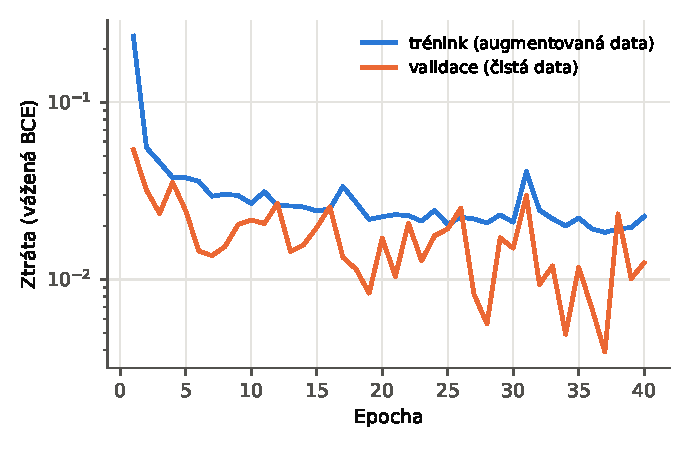
\includegraphics[width=\linewidth]{cnn_uceni.pdf}\end{minipage}\hfill
\begin{minipage}{0.56\textwidth}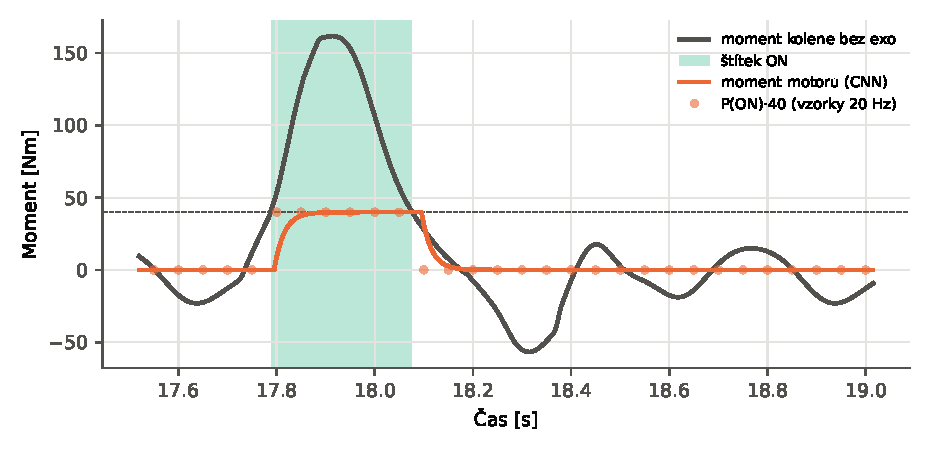
\includegraphics[width=\linewidth]{cnn_detail_kroku.pdf}\end{minipage}
\caption{Vlevo: průběh učení. Vpravo: detail jednoho kroku na schodech v testovací části.
Šedý průběh je potřebný moment kolene, zelená plocha štítek ON, body výstup sítě (20\,Hz)
a oranžová čára výsledný moment motoru.}
\end{figure}

\subsection{Výsledky klasifikace}
\begin{table}[H]
\centering\small
\begin{tabular}{lcccc}
\toprule
Testovací podmínky (jen testovací úseky) & přesnost & precision & recall & F1\\
\midrule
čistá data & \CnnCistaAcc & \CnnCistaPrec & \CnnCistaRec & \CnnCistaF\\
dvojnásobný šum snímačů & \CnnSumAcc & \CnnSumPrec & \CnnSumRec & \CnnSumF\\
pomalejší chůze ($-15$\pct) & \CnnPomalaAcc & \CnnPomalaPrec & \CnnPomalaRec & \CnnPomalaF\\
rychlejší chůze ($+15$\pct) & \CnnRychlaAcc & \CnnRychlaPrec & \CnnRychlaRec & \CnnRychlaF\\
\bottomrule
\end{tabular}
\caption{Kvalita rozhodování na 20\,Hz vzorcích testovací množiny.
Precision = podíl zapnutí, která byla správně; recall = podíl potřebných zapnutí, která síť zachytila.}
\end{table}

\begin{figure}[H]
\centering
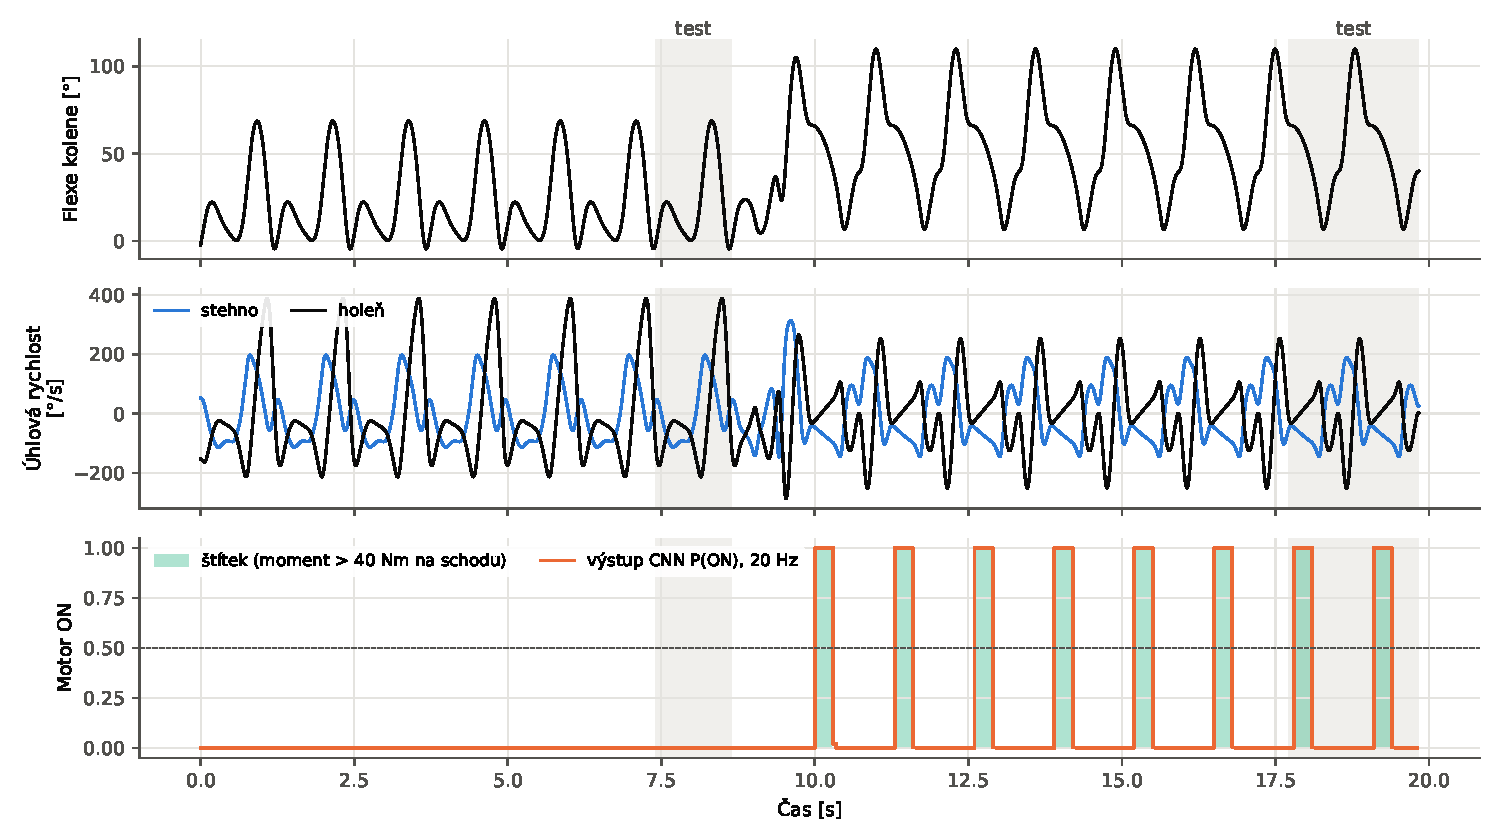
\includegraphics[width=\textwidth]{cnn_prubeh.pdf}
\caption{Vstupy sítě a její výstup za celých 15\,m. Šedě jsou vyznačené testovací úseky.
Na rovině zůstává výstup nulový. Na schodech se síť zapíná v každém kroku a kryje se se štítkem.}
\end{figure}

V uzavřené smyčce se síť zapnula v průměru \CnnZpozdeniOn\,ms po štítku a vypnula
\CnnZpozdeniOff\,ms po něm. To je dáno 20\,Hz vzorkováním (krok 50\,ms). Na rovině nebylo
žádné falešné zapnutí (\CnnFalesna). Pozor: vysoké skóre je potřeba brát s rezervou, protože
data obsahují jediný typ chůze po rovině a jediný (syntetický) styl výstupu do schodů.
Před nasazením je nutné síť ověřit na naměřených datech více osob, s jinými schody
a s jinými přechody (rovina → schody, zastavení, otočka, chůze ze schodů).

%==========================================================================
\section{Odlehčení kolene}\label{sec:vysledky}

Srovnává se pět variant:
\emph{bez exo} (výsledek z test1);
\emph{pasivní exo} (jen hmotnost, motor vypnutý);
\emph{úhel + směr} (dřívější řízení, moment $G(\theta)$ vyladěný podle úhlu kolene,
jen při natahování kolene, max. 60\Nm);
\emph{CNN} (tato zpráva, ON/OFF 40\Nm);
\emph{ideální ON/OFF} (motor spíná přesně podle štítku, bez zpoždění rozhodnutí).
Moment, který musí dodat člověk, se počítá podle rovnice~\eqref{eq:superpozice}.

\begin{figure}[H]
\centering
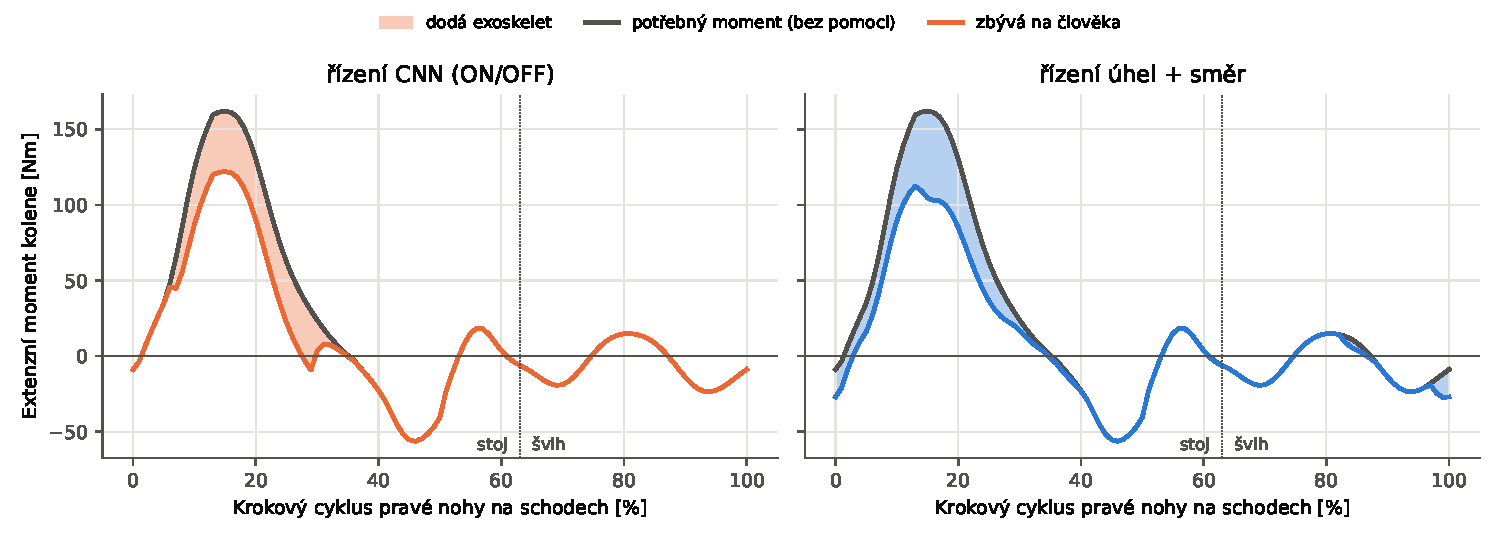
\includegraphics[width=\textwidth]{odlehceni_schody.pdf}
\caption{Moment kolene při výstupu do schodů (průměr 6 kroků, 0\pct{} = dopad pravé nohy na schod).
Šedá je potřebný moment, barevná čára je podíl člověka a vybarvená plocha je to, co převezme
exoskelet. Barva odpovídá řízení (oranžová CNN, modrá úhel + směr).}
\label{fig:odlehceni}
\end{figure}

\begin{figure}[H]
\centering
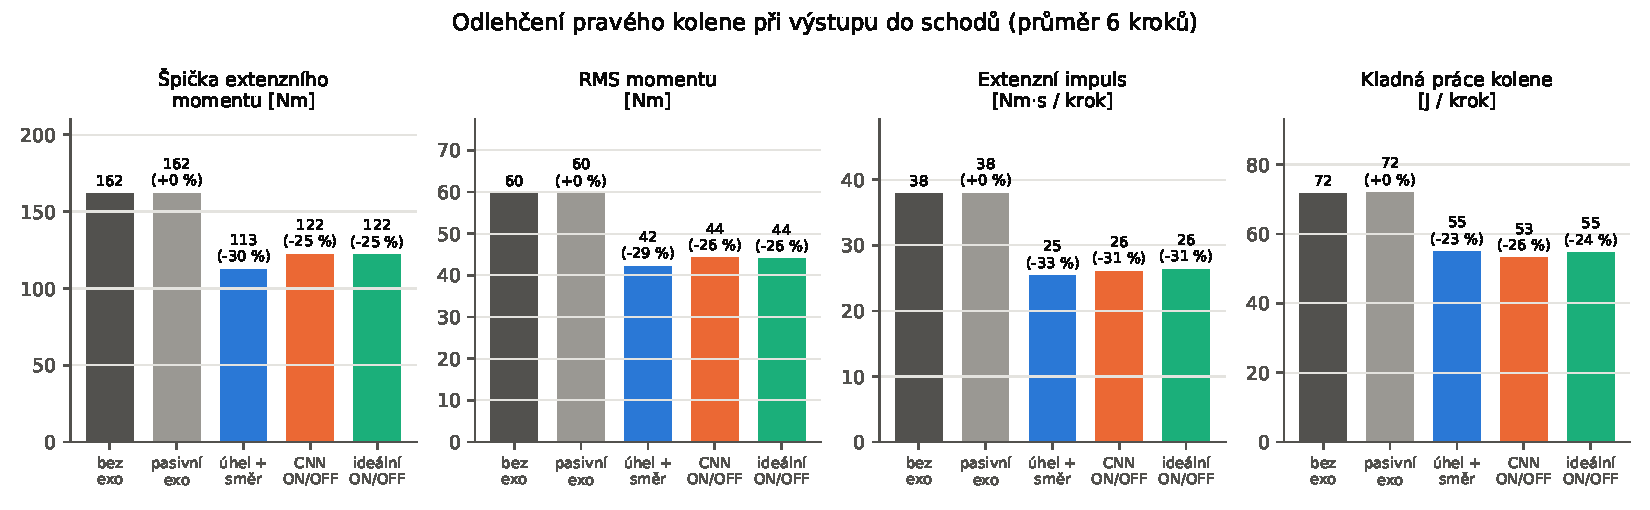
\includegraphics[width=\textwidth]{odlehceni_sloupce.pdf}
\caption{Souhrnné ukazatele zatížení kolene na schodech. Procenta jsou změna proti chůzi bez exoskeletu.
Extenzní impuls je plocha pod kladnou částí momentu za jeden krok.}
\label{fig:sloupce}
\end{figure}

\begin{table}[H]
\centering\small
\begin{tabular}{lrrrrr}
\toprule
Schody, průměr na krok & bez exo & pasivní & úhel + směr & \textbf{CNN} & ideální ON/OFF\\
\midrule
špička extenzního momentu [N\,m] & \SchodyBezSpicka & \SchodyPasSpicka & \SchodyUhelSpicka & \textbf{\SchodyCnnSpicka} & \SchodyIdealSpicka\\
RMS momentu [N\,m] & \SchodyBezRms & \SchodyPasRms & \SchodyUhelRms & \textbf{\SchodyCnnRms} & \SchodyIdealRms\\
extenzní impuls [N\,m\,s] & \SchodyBezImpuls & \SchodyPasImpuls & \SchodyUhelImpuls & \textbf{\SchodyCnnImpuls} & \SchodyIdealImpuls\\
kladná práce svalů kolene [J] & \SchodyBezPrace & \SchodyPasPrace & \SchodyUhelPrace & \textbf{\SchodyCnnPrace} & \SchodyIdealPrace\\
flexní špička [N\,m] & \SchodyBezFlex & \SchodyPasFlex & \SchodyUhelFlex & \textbf{\SchodyCnnFlex} & \SchodyIdealFlex\\
\midrule
práce motoru [J] & -- & -- & \SchodyUhelExoPrace & \textbf{\SchodyCnnExoPrace} & \SchodyIdealExoPrace\\
max. výkon motoru [W] & -- & -- & \SchodyUhelExoVykon & \textbf{\SchodyCnnExoVykon} & \SchodyIdealExoVykon\\
\bottomrule
\end{tabular}
\caption{Zatížení pravého kolene při výstupu do schodů.}
\label{tab:vysledky}
\end{table}

\paragraph{Interpretace.}
\begin{itemize}
  \item Řízení CNN sníží špičku extenzního momentu o \SchodyCnnSpickaRed\pct{}
        (o 40\Nm, tedy přesně o moment motoru), extenzní impuls o \SchodyCnnImpulsRed\pct{}
        a kladnou práci svalů kolene o \SchodyCnnPraceRed\pct. Exoskelet dodá
        \SchodyCnnExoPrace\,J na krok při špičkovém výkonu \SchodyCnnExoVykon\,W.
  \item CNN je prakticky stejně dobrá jako ideální ON/OFF s okamžitým spínáním.
        Zpoždění rozhodnutí 10--20\,ms se při době zapnutí asi 300\,ms projeví jen málo.
  \item Řízení „úhel + směr“ dává na schodech podobné odlehčení (vyšší motor, až 60\Nm).
        Na rovině ale škodí, protože ve švihu tlačí koleno do extenze (obr.~\ref{fig:rovina}).
        Úhel kolene sám neodliší stoj na schodu od švihu. CNN to díky úhlovým rychlostem segmentů
        a historii za 1\,s dokáže.
  \item Flexní špička (\SchodyCnnFlex\Nm) se nezměnila. Motor působí jen v době velkého
        extenzního momentu, nikde proti člověku.
  \item Kyčel a kotník: momenty se nemění, protože pohyb je předepsaný a moment motoru působí
        mezi stehnem a bércem. Jejich nepatrné změny způsobuje jen hmota exoskeletu.
\end{itemize}

\begin{figure}[H]
\centering
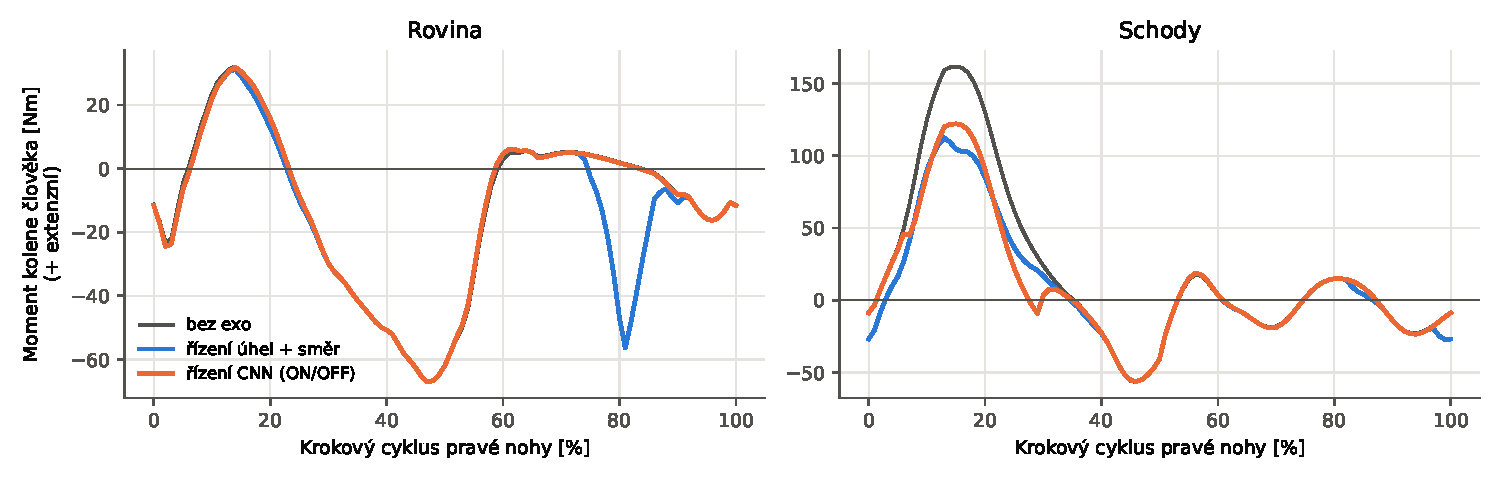
\includegraphics[width=\textwidth]{rovina_vs_schody.pdf}
\caption{Moment kolene člověka na rovině a na schodech. Na rovině se CNN nezapne a průběh je
totožný s chůzí bez exoskeletu. Řízení podle úhlu na rovině přidává flexní moment ve švihu.}
\label{fig:rovina}
\end{figure}

\begin{figure}[H]
\centering
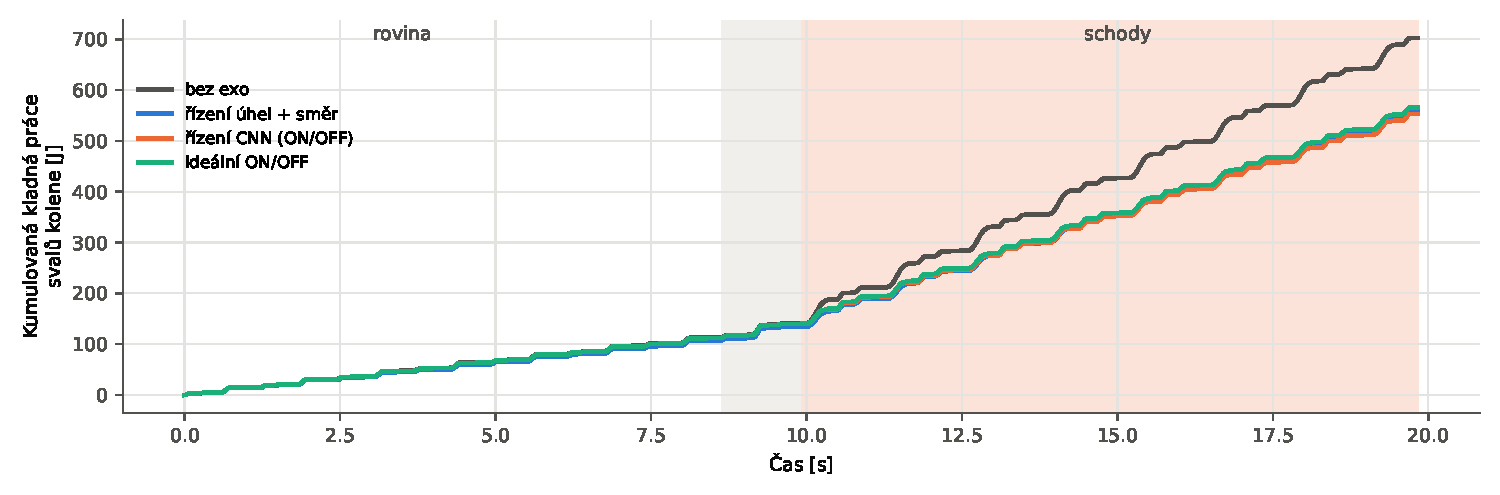
\includegraphics[width=\textwidth]{kumulativni_prace.pdf}
\caption{Kumulovaná kladná práce svalů kolene za celých 15\,m. Na rovině se křivky nerozcházejí.
Na schodech exoskelet s řízením CNN ušetří asi 19\,J v každém kroku pravé nohy.}
\end{figure}

\paragraph{Požadavky na pohon (CNN, ON/OFF).} Moment 40\Nm, špičkový výkon asi 100\,W a
rychlost kolene při zapnutém motoru do 3\,rad/s. Dimenzování z CAD (BLDC motor + vlnový převod,
vrcholový moment 60\Nm) tedy vyhovuje s rezervou.

%==========================================================================
\section{Animace chůze}\label{sec:animace}

Video \texttt{results/animace/chuze\_exo\_email.mp4} (H.264, 1280×720, 25\,snímků/s, 19,8\,s, 2\,MB) ukazuje celý
průchod 15\,m. Kamera sleduje pánev modelu: posouvá se s chůzí vpřed i nahoru po schodech
a dívá se z pravé strany mírně zezadu, aby byl exoskelet vidět. Vlevo je kostra modelu
s exoskeletem a reakční síly země (šipky, 1\,m = 1000\,N). Vpravo běží posuvné grafy
flexe kolene, momentu kolene (bez exo / člověk s exo) a momentu motoru s vyznačeným stavem
ON. Snímky se kreslí z poloh těles spočtených v OpenSim.

\begin{figure}[H]
\centering
\begin{subfigure}{0.49\textwidth}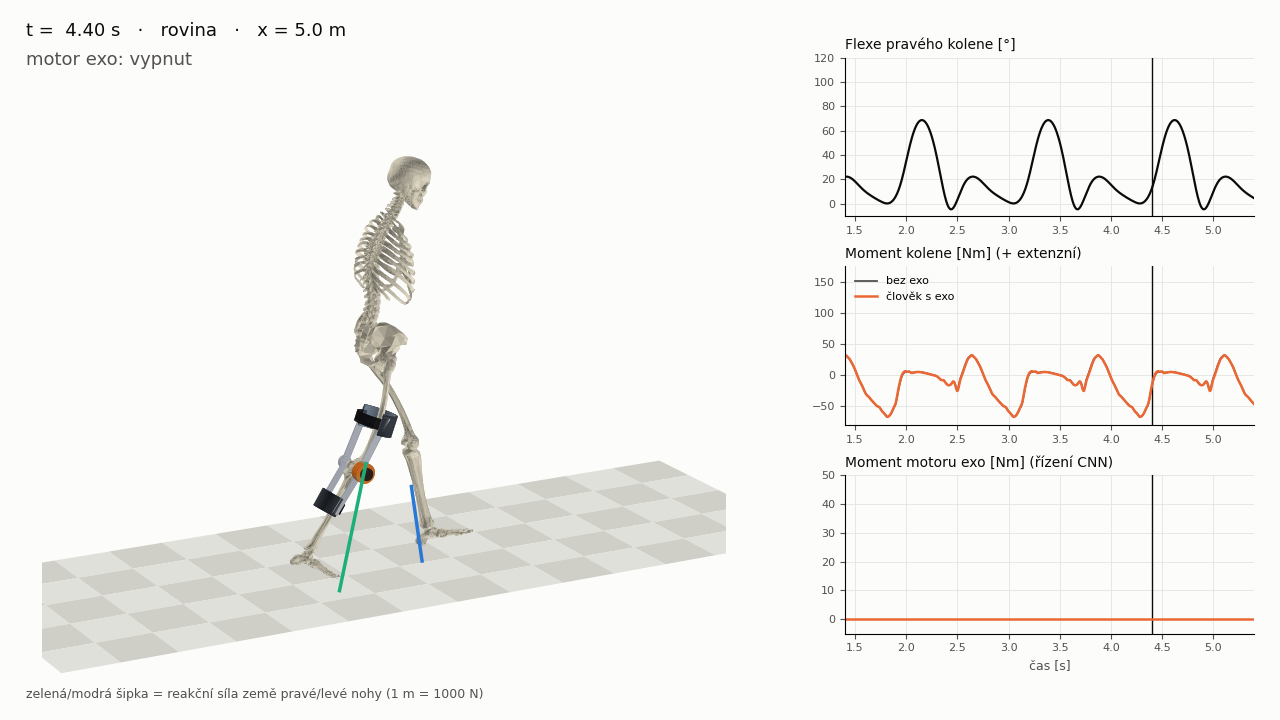
\includegraphics[width=\linewidth]{snimek_rovina.png}\caption{rovina}\end{subfigure}\hfill
\begin{subfigure}{0.49\textwidth}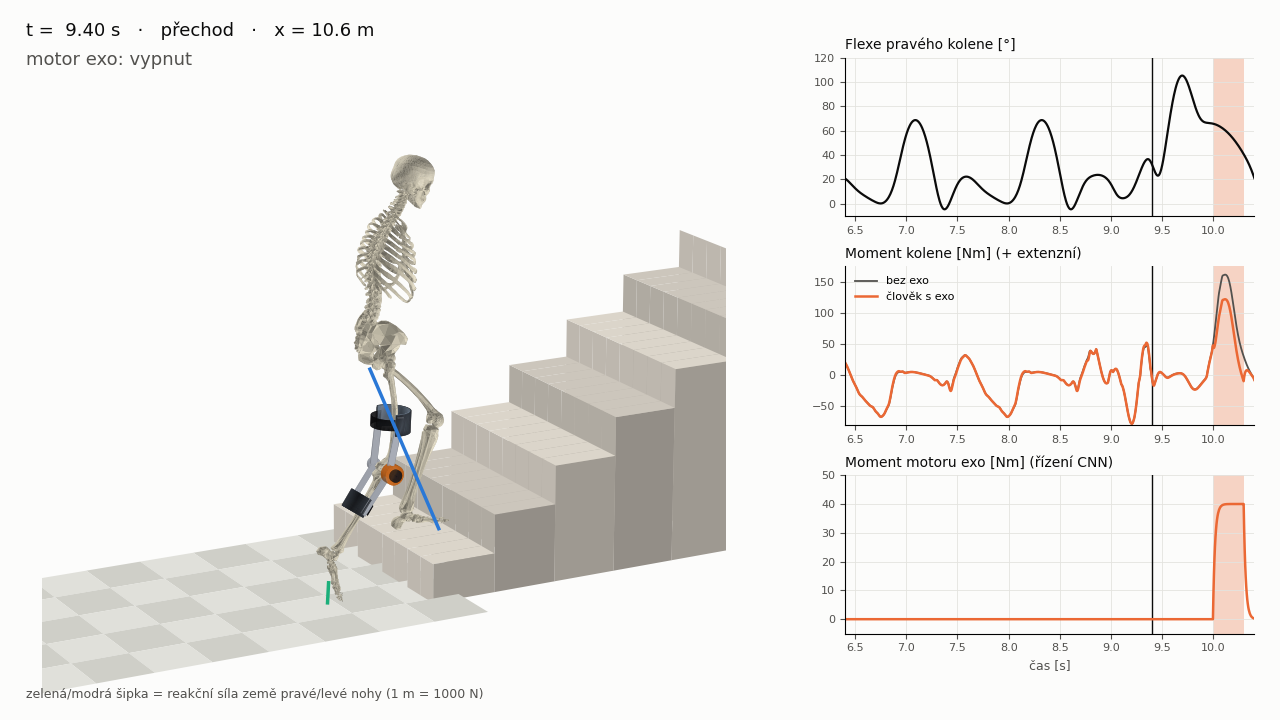
\includegraphics[width=\linewidth]{snimek_prechod.png}\caption{přechod na schody}\end{subfigure}\\[4pt]
\begin{subfigure}{0.49\textwidth}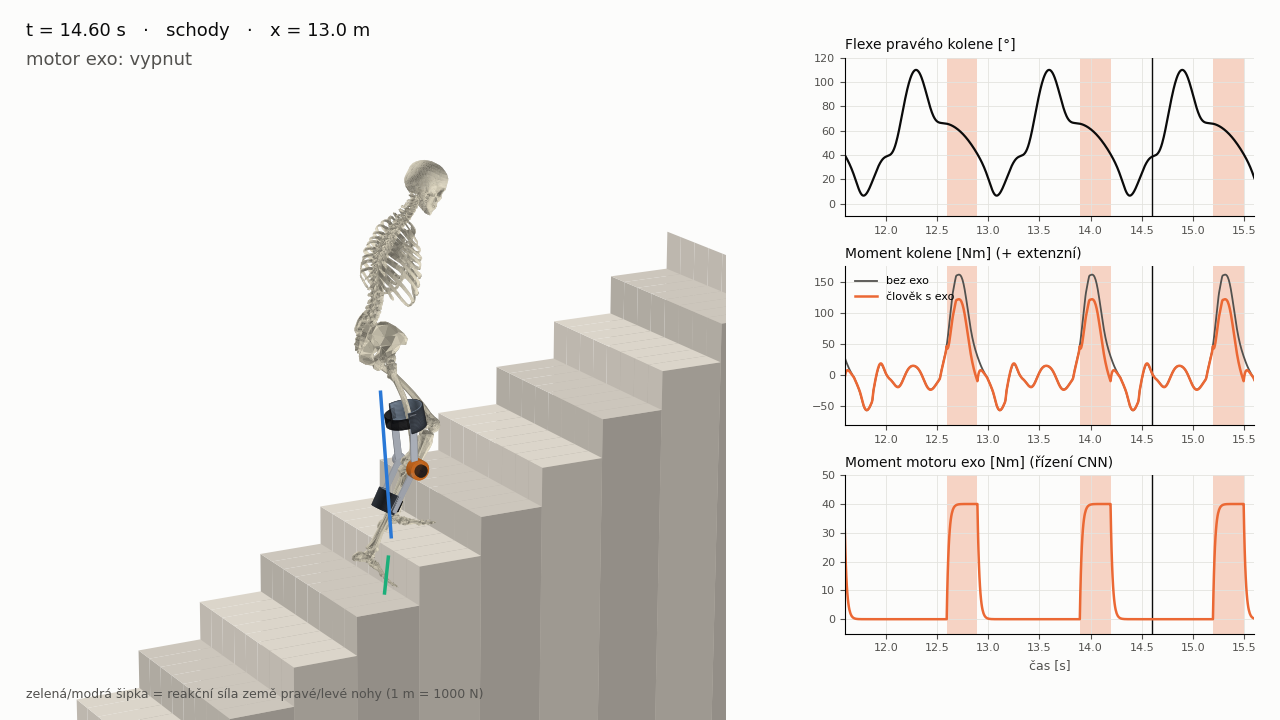
\includegraphics[width=\linewidth]{snimek_schody_stoj.png}\caption{schody}\end{subfigure}\hfill
\begin{subfigure}{0.49\textwidth}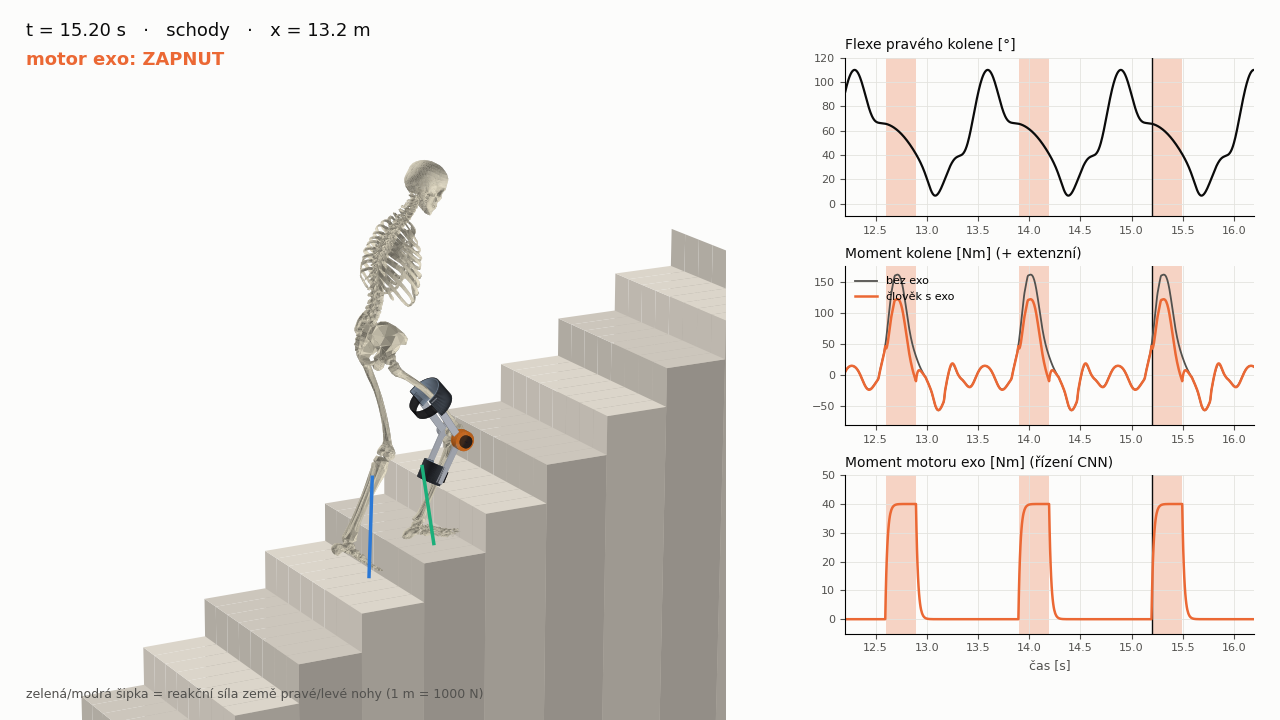
\includegraphics[width=\linewidth]{snimek_schody_svih.png}\caption{schody, další fáze kroku}\end{subfigure}
\caption{Snímky z animace.}
\end{figure}

%==========================================================================
\section{Omezení a doporučení}
\begin{itemize}
  \item \textbf{Předepsaný pohyb.} Výsledky platí za předpokladu, že člověk s exoskeletem chodí stejně.
        Adaptaci pohybu by ukázala až dopředná simulace se svaly (OpenSim Moco).
  \item \textbf{Čisté momenty, ne svalové síly.} Odlehčení je vyjádřeno momentem a prací v koleni.
        Jak se zmenší síla čtyřhlavého svalu nebo tlak v kloubu, by ukázala statická optimalizace.
  \item \textbf{Data pro CNN} pocházejí z jedné osoby. Rovina je jeden zopakovaný naměřený cyklus,
        schody jsou syntetické. Augmentace pomáhá s robustností vůči šumu a rychlosti, ale
        naměřená data nenahradí. Doporučuje se sběr dat s IMU a enkodérem na skutečném prototypu
        a doučení sítě.
  \item \textbf{Bezpečnost.} V praxi je potřeba omezit dobu zapnutí (například 0,6\,s), zakázat
        zapnutí při natažené noze a doplnit tlačítko nebo detekci, která exoskelet vypne.
  \item \textbf{Ideální pohon a tuhé objímky.} Chybí tření a setrvačnost motoru, poddajnost
        měkkých tkání a dynamika regulace proudu. Pro ON/OFF řízení by se hodilo plynulé
        zvyšování momentu (rampa), které omezí rázy.
  \item \textbf{Možné rozšíření:} místo ON/OFF regrese momentu stejnou sítí, tedy výstup
        $\tau\in[0, 60]$\Nm. Moment by pak sledoval průběh potřeby (obr.~\ref{fig:odlehceni})
        a mohl by snížit i špičku, kterou ON/OFF se 40\Nm{} snižuje jen o 40\Nm.
\end{itemize}

%==========================================================================
\appendix
\section{Soubory a spuštění}
\small
\begin{tabularx}{\textwidth}{l>{\raggedright\arraybackslash}X}
\toprule
\texttt{model/subject01\_stairs\_exo.osim} & model s exoskeletem pro OpenSim GUI\\
\texttt{cad/} & STL díly (mm), sestava, kusovník, náhledy\\
\texttt{scripts/cnn\_train.py} & učení sítě (Python 3.11 + PyTorch)\\
\texttt{scripts/cnn\_rizeni.py} & řízení CNN pro smyčku 20\,Hz (numpy)\\
\texttt{scripts/run\_moje\_rizeni.py} & vyhodnocení libovolného řízení (\texttt{cnn\_rizeni}, \texttt{moje\_rizeni})\\
\texttt{scripts/anim\_export.py}, \texttt{anim\_render.py} & animace (OpenSim → snímky → MP4)\\
\texttt{scripts/zprava\_grafy.py} & grafy a čísla této zprávy\\
\texttt{results/cnn/} & váhy sítě (\texttt{cnn\_vahy.npz}, \texttt{cnn\_model.pt}), metriky\\
\texttt{results/animace/chuze\_exo\_email.mp4} & video (H.264)\\
\bottomrule
\end{tabularx}

\medskip
\noindent Pořadí výpočtu (\texttt{PY38} = Python 3.8 s OpenSim, \texttt{PY311} = Python 3.11 s PyTorch):
\begin{verbatim}
PY38  exo_cad.py ; PY38 build_exo_model.py ; PY38 run_exo.py
PY311 cnn_train.py ; PY38 run_moje_rizeni.py cnn_rizeni
PY38  anim_export.py ; PY311 anim_render.py ; PY311 zprava_grafy.py
xelatex zprava_exoskelet.tex   (2x)
\end{verbatim}

\end{document}
